\section{Auswertung}
\label{sec:Auswertung}

Die für die verschiedenen Heizströme $I_{\text{Heiz}}$ bzw. Heizspannung $U_{\text{Heiz}}$ gemessenen Werte sind in den Tabellen (\ref{tab:Kennlinie_1_2}),
(\ref{tab:Kennlinie_3_4}) und (\ref{tab:Kennlinie_5}) aufgetragen. Die verschiedenen Kennlinien sind in den Abbildungen (\ref{fig:plot_1}) und (\ref{plot_2}) dargestellt. 

\begin{table}[H]
    \centering
    \caption{Gemessener Strom in Abhängigkeit von der Spannung bei $I_{\text{Heiz}} = 2$ und $U_{\text{Heiz}} = 4$ in den linken beiden Spalten und bei $I_{\text{Heiz}} = 2.1$ und $U_{\text{Heiz}} = 4$ in den rechten beiden Spalten.}
    \label{tab:Kennlinie_1_2}
    \begin{tblr}{colspec={c c || c c}}
        \toprule
        $\text{Spannung} \left[\unit{\volt}\right]$ & $\text{Strom} \left[\unit{\milli\ampere}\right]$ & $\text{Spannung} \left[\unit{\volt}\right]$ & $\text{Strom} \left[\unit{\milli\ampere}\right]$ \\
        \midrule  
        10    &  0,013  &   15    &  0,032 \\
        20    &  0,029  &   30    &  0,072 \\
        30    &  0,043  &   40    &  0,096 \\
        40    &  0,050  &   50    &  0,111 \\
        50    &  0,054  &   60    &  0,121 \\
        60    &  0,056  &   70    &  0,121 \\
        70    &  0,056  &   80    &  0,126 \\
        80    &  0,057  &   90    &  0,130 \\
        90    &  0,059  &   100   &  0,133 \\
        100   &  0,059  &   110   &  0,134 \\
        110   &  0,060  &   120   &  0,135 \\
              &         &   130   &  0,136 \\
              &         &   140   &  0,137 \\
              &         &   150   &  0,128 \\
              &         &   160   &  0,139 \\
              &         &   170   &  0,140 \\
              &         &   180   &  0,140 \\
             
        \bottomrule
    \end{tblr}
\end{table}

\begin{table}[H]
    \centering
    \caption{Gemessener Strom in Abhängigkeit von der Spannung bei $I_{\text{Heiz}} = 2,2$ und $U_{\text{Heiz}} = 4,5$ in den linken beiden Spalten und bei $I_{\text{Heiz}} = 2.3$ und $U_{\text{Heiz}} = 5$ in den rechten beiden Spalten.}
    \label{tab:Kennlinie_3_4}
    \begin{tblr}{colspec={c c || c c}}
        \toprule
        $\text{Spannung} \left[\unit{\volt}\right]$ & $\text{Strom} \left[\unit{\milli\ampere}\right]$ & $\text{Spannung} \left[\unit{\volt}\right]$ & $\text{Strom} \left[\unit{\milli\ampere}\right]$\\
        \midrule  
        10      &       0,026 & 15      &       0,052\\
        20      &       0,060 & 30      &       0,128\\
        30      &       0,101 & 45      &       0,214\\
        40      &       0,146 & 60      &       0,306\\
        50      &       0,189 & 75      &       0,402\\
        60      &       0,227 & 90      &       0,491\\
        70      &       0,250 & 105     &       0,557\\
        80      &       0,274 & 120     &       0,609\\
        90      &       0,289 & 135     &       0,644\\
        100     &       0,298 & 150     &       0,667\\
        110     &       0,309 & 165     &       0,683\\
        120     &       0,310 & 180     &       0,694\\
        130     &       0,314 & 195     &       0,702\\
        140     &       0,316 & 210     &       0,709\\
        150     &       0,319 & 225     &       0,714\\
                &             & 240     &       0,719\\
        \bottomrule
    \end{tblr}
\end{table}


\begin{table}[H]
    \centering
    \caption{Gemessener Strom in Abhängigkeit von der Spannung bei $I_{\text{Heiz}} = 2.4$ und $U_{\text{Heiz}} = 5$.}
    \label{tab:Kennlinie_5}
    \begin{tblr}{colspec={c c}}
        \toprule
        $\text{Spannung} \left[\unit{\volt}\right]$ & $\text{Strom} \left[\unit{\milli\ampere}\right]$ \\
        \midrule  
        3       & 0,007\\
        6       & 0,017\\
        9       & 0,027\\
        12      & 0,040\\
        15      & 0,053\\
        18      & 0,067\\
        21      & 0,081\\
        24      & 0,098\\
        27      & 0,114\\
        30      & 0,129\\
        33      & 0,149\\
        36      & 0,171\\
        39      & 0,193\\
        42      & 0,214\\
        45      & 0,235\\
        48      & 0,251\\
        51      & 0,275\\
        54      & 0,299\\
        57      & 0,322\\
        60      & 0,352\\
        65      & 0,400\\
        70      & 0,441\\
        75      & 0,492\\
        80      & 0,535\\
        85      & 0,576\\
        90      & 0,626\\
        110     & 0,786\\
        130     & 0,930\\
        150     & 1,053\\
        170     & 1,158\\
        190     & 1,238\\
        210     & 1,292\\
        230     & 1,330\\
        250     & 1,356\\
        \bottomrule
    \end{tblr}
\end{table}

\begin{figure}
    \centering
    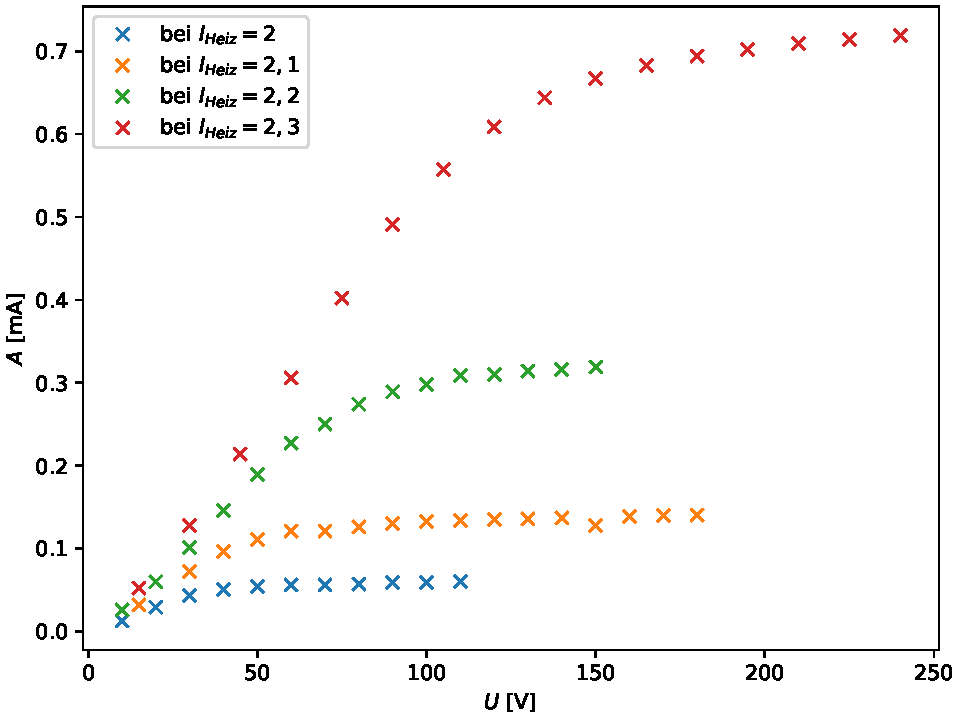
\includegraphics[width=\textwidth]{plot_1.pdf}
    \caption{Kennlinien der Diode bei verschiedenen Heizströmen.}
    \label{fig:plot_1}
\end{figure}
\begin{figure}
      \centering
      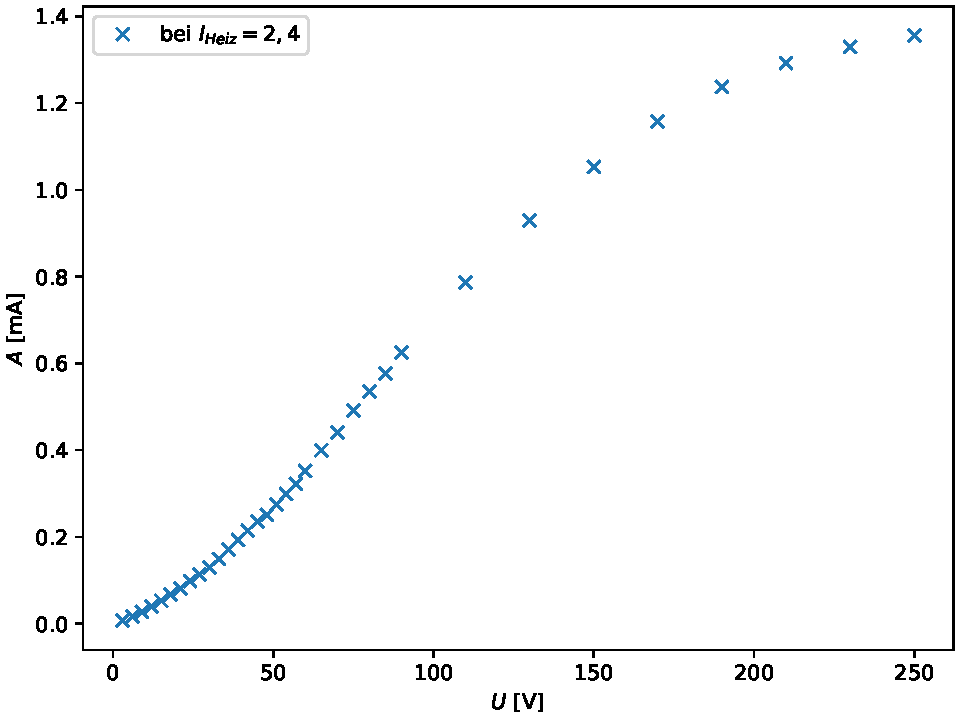
\includegraphics[width=\textwidth]{plot_2.pdf}
      \caption{Kennlinien der Diode bei einem Heizstrom von 2,4 mA}
      \label{fig:plot_2}
\end{figure}
\begin{table}[H]
    \centering
    \caption{Gemessener Strom in Abhängigkeit von der Spannung bei $I_{\text{Heiz}} = 2.4$ und $U_{\text{Heiz}} = 5$.}
    \label{tab:Kennlinie_5}
    \begin{tblr}{colspec={c c}}
        \toprule
        $I_{\text{Heiz}} \left[\unit{\milli\ampere}\right]$ & $I_{S} \left[\unit{\milli\ampere}\right]$ \\
        \midrule  
        2,0 &  0,060 \\
        2,1 &  0,140 \\
        2,2 &  0,319 \\
        2,3 &  0,719 \\
        3,4 &  1,356 \\
        \bottomrule
    \end{tblr}
\end{table}
Aus den Abbidlungen (\ref{fig:plot_1}) und (\ref{fig:plot_2}) werden die Sättigungsströme $I_S$ abgelesen, die in Tabelle (\ref{tab:Kennlinie_5}) aufgelistet sind.

\subsection{Gültigkeit des Langmuir-Schottkyschen Raumladungsgesetzes}
Die Langmuir-Schottkysche Gleichung (\ref{}) hat die Form $I = a \cdot U^b$. Diese lässt sich durch Logarithmisieren 
in die Geradengleichung 
    \begin{equation*}
    \log(I) = b \cdot \log(U) + \log(a)
    \end{equation*}
bringen. Zur Überprüfung der Gleichung wird eine lineare Regression der 5. Kennlinie verwendet, die bei dem 
höchsten Heizstrom entsteht. Die Regression und die Messwerte der 5. Kennlinie sind in Abbildung (\ref{fig:plot_3}) abgebildet. 
\begin{figure}
    \centering
    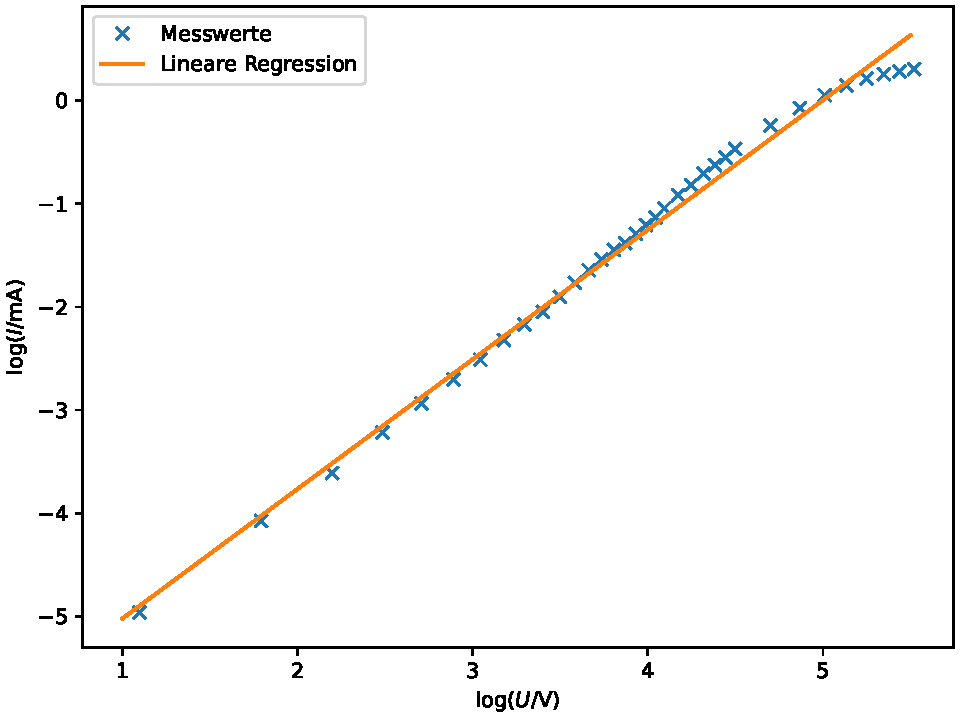
\includegraphics[width=\textwidth]{plot_3.pdf}
    \caption{Lineare Regression der logarithmisierten, fünften Kennlinie.}
    \label{fig:plot_3}
\end{figure}

Durch die lineare Regression ergeben sich 
die Werte
\begin{align}
    \log(a) &= 1,26 \pm 0,02 \\
    b &= -6,28 \pm 0,08 \, .
\end{align}
$b$ ist zur Auswertung der Gültigkeit nicht relevant. $\log(a)$ kann mit dem Theoriewert $\log(a)_{\text{Theo}}= \frac{3}{2}$ verglichen werden.

\subsection{Bestimmung der Kathodentemperatur}
Der Bereich des Anlaufstroms hat einen exponentiellen Zusammenhang zwischen Strom und 
Spannung wie in Gleichung (\ref{}) zu sehen ist. Durch das Logarithmieren des Stroms 
und dem Auftragen gegen die Spannung eine lineare Regression der Form 
$$y = cx + d$$
durchgeführt werden. Die verwendeten Messwerte aus dem Anlaufbereich sind in Tabelle (\ref{tab:Anlaufbereich}) zu sehen. 
\begin{table}[H]
    \centering
    \caption{Gemessener Strom in Abhängigkeit von der Spannung im Anlaufbereich.}
    \label{tab:Anlaufbereich}
    \begin{tblr}{colspec={c c}}
        \toprule
        $\text{Spannung} \left[\unit{\volt}\right]$ & $\text{Strom} \left[\unit{\nano\ampere}\right]$ \\
        \midrule  
        0       & 4,40 \\
        0,05    & 3,00 \\
        0,1     & 2,10 \\
        0,15    & 1,90 \\
        0,2     & 1,45 \\
        0,25    & 1,00 \\
        0,3     & 0,79 \\
        0,4     & 0,40 \\
        0,5     & 0,185 \\
        0,6     & 0,059 \\
        0,65    & 0,014 \\
        \bottomrule
    \end{tblr}
\end{table}
Diese Messwerte und die lineare Rgression sind in Abbildung (\ref{}) dargestellt. 
\begin{figure}
    \centering
    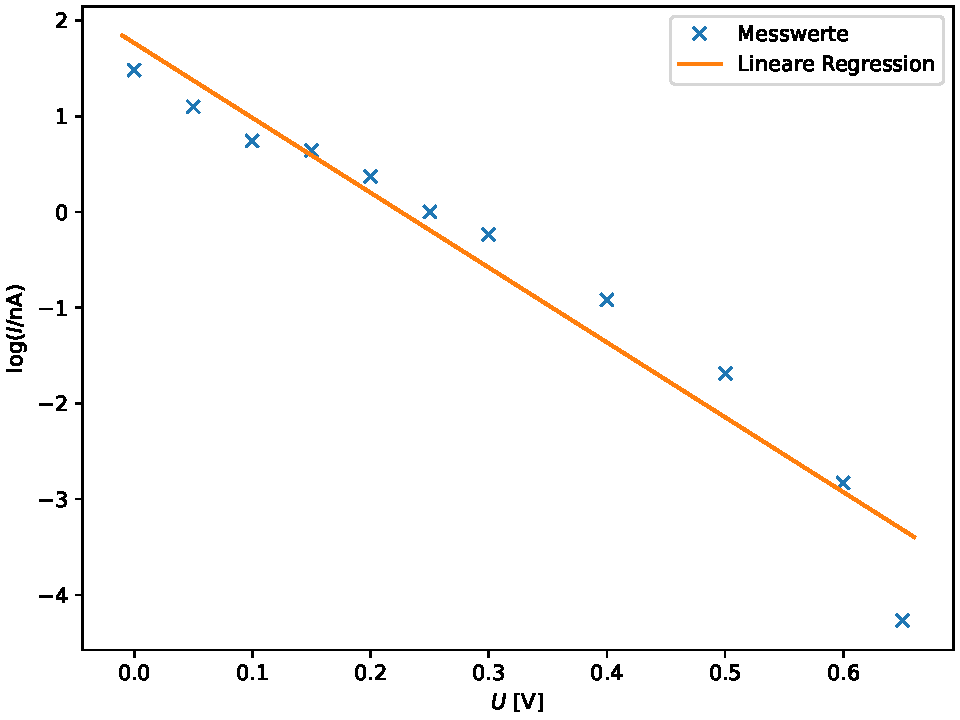
\includegraphics[width=\textwidth]{plot_4.pdf}
    \caption{Lineare Regression der messwerte aus dem Anlaufbereich.}
    \label{fig:plot_3}
\end{figure}
Die Wert der lineare Regression bestimmen sich zu 
\begin{align*}
    c &= -7,8 \pm 0,6 \\
    d &= 1,7 \pm 0,2 \, .
\end{align*}
Durch Vergleich mit Gleichung (\ref{}) ergibt sich 
\begin{align*}
    c &= -\frac{e}{kT} \\
    \Leftrightarrow T &= -\frac{e}{kc}
\end{align*}
für die Kathodentemperatur $T$. 
Die aus den Messwerten bestimmte Kathodentemperatur ist 
$$ T = (1,5 \pm 0,1)\cdot 10^{3} \, \, \unit{\kelvin}\,.$$

\subsection{Bestimmung der Kathodentemperaturen und Austrittsarbeit von Wolfram}

%Siehe \autoref{fig:plot}!